\section{Durchführung}
\label{sec:Durchfuehrung}

\begin{figure}
    \centering
    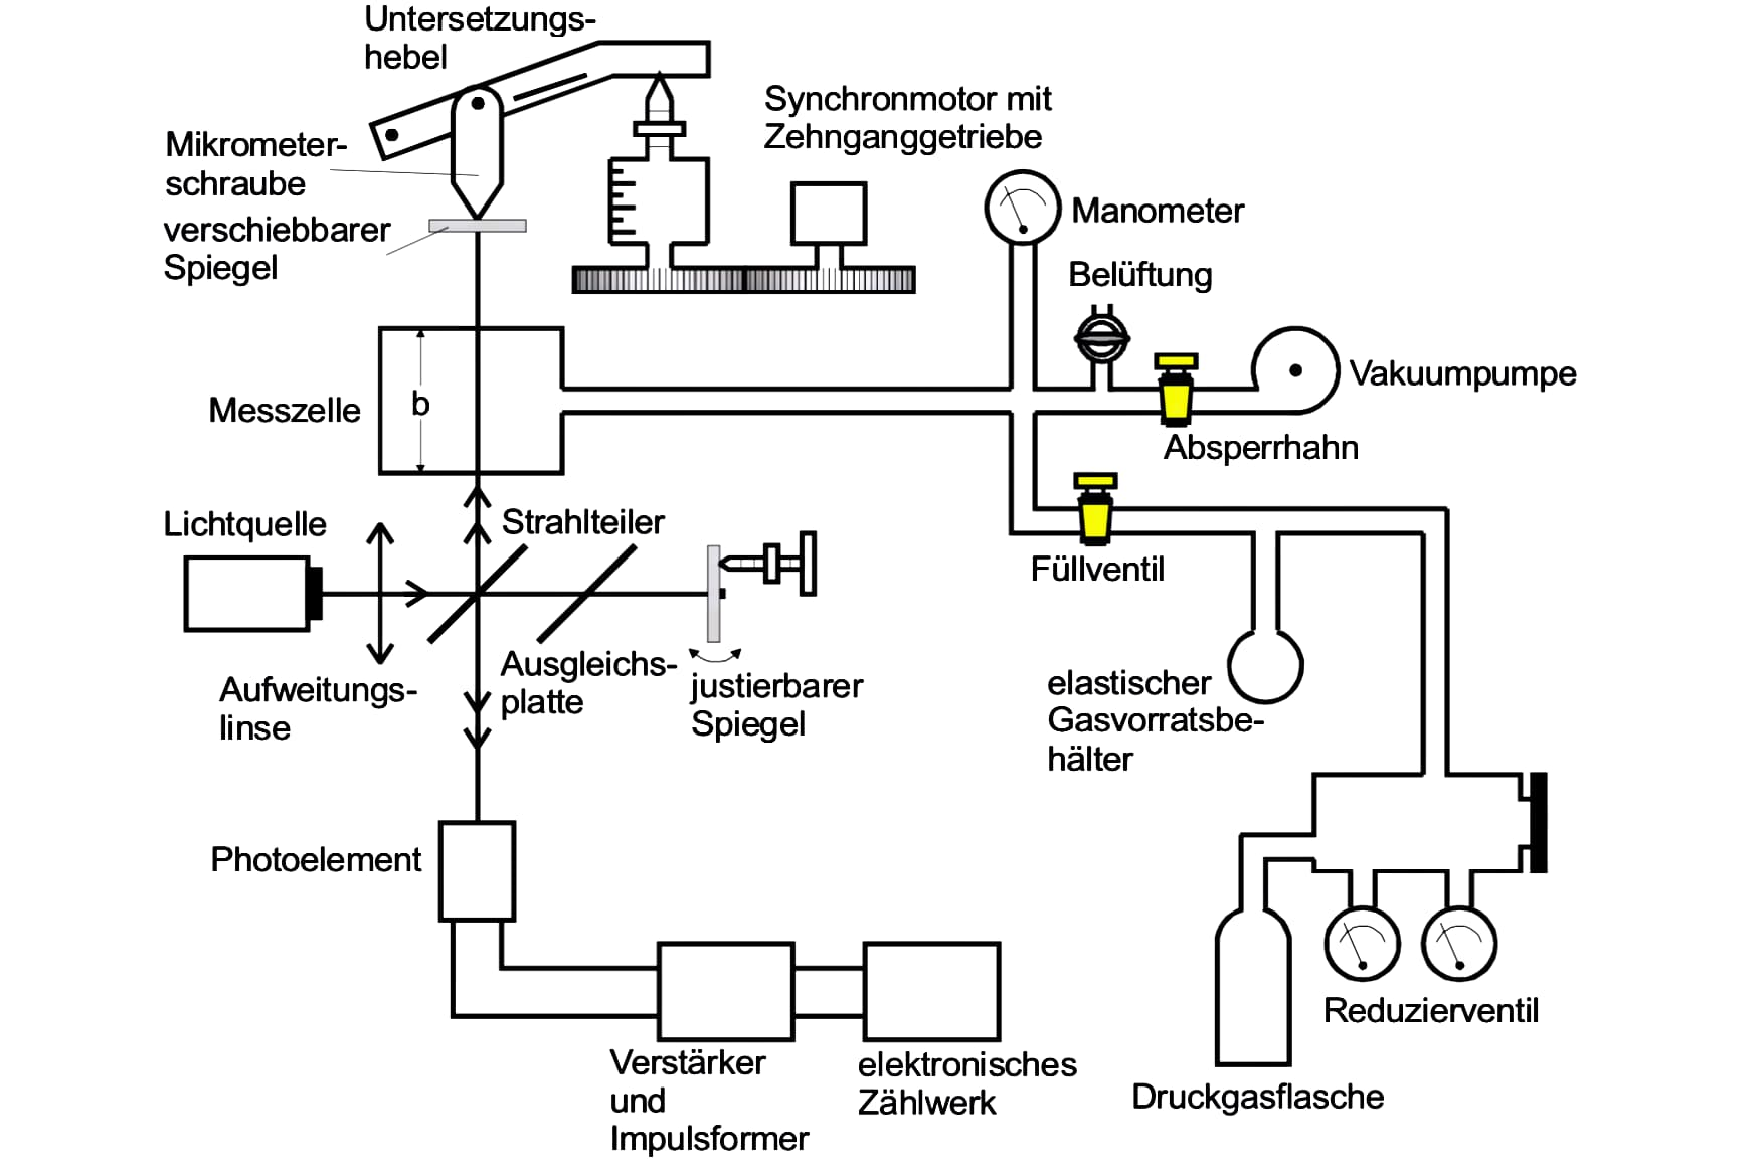
\includegraphics[scale = 0.5]{content/Aufbau1.pdf}
    \caption{Hier zu sehen ist eine Skizze zum Aufbau des Versuchs.}
    \label{fig:Teiler}
\end{figure}

Um erstmal die Wellenlänge des Lasers zu bestimmen, wird der Spiegel konstant verschoben. Dabei werden die Maxima mit dem Photoelement gezählt. Dies geht so lange weiter bis die Anzahl der gezählten Maxima in etwa 3100 erreicht. Die Verschiebung des Spiegels in dem Zeitraum wird als \(d\) eingetragen.\\
Danach wird der Brechungsindex gemessen. Bei Luft wird die Messzelle evakuiert, wodurch der Druck steigt. Dann wird wieder Luft reingelassen und das Prozedere wiederholt, nachdem der Druck danach wieder als Normaldruck aufgeschrieben wird.\\
Die Messungen werden fünf mal durchgeführt, sodass das Ergebnis genauer ist.